%\newpage
\section{Measurement of Semiconductors}
One probe pin is assumed to be the negative side of the component.
Another pin is assumed to be the positive side of the component.
For a first test, the components positive side is directly connected to VCC.
The negative side is connected with the \(680\Omega\) resistor to GND.
The test probe (third pin, also called TriStatePin) is first connected with the \(680\Omega\) resistor
for 10 ms to GND. The voltage of the negative probe pin is read, during  the TriStatePin is
switched to Input (High Impedance). It is assumed that the tested part can be
a N-Channel MOSFET and the gate should be discharged.
If the readed voltage is above 976mV, the next test assume, that the tested part can
also be a P-Channel MOSFET and for this a 10ms switch of the TriStatePin with the \(680\Omega\) resistor
to the VCC side is done.
Also for this case the voltage at the negative Probe Pin is read.
If the voltage of the negative Pin is greater than 92mV with the
currentless TriStatePin, additional tests are made to differ N-Channel JFET or D-MOSFET (depletion)
and P-Channel JFET or P-MOSFET. MOSFET versions can be differed by the missing of current in any state
of the TriStatePin.
If the component has no current between positive probe and negative probe without signal at the
TristatePin, the next tests are specified in the next section \ref{sec:pnp}.
If current was detected, the next test is described in the diode section \ref{sec:diode}.

\subsection{Measurement of PNP Transistor or P-Channel-MOSFET}
\label{sec:pnp}
First the current amplification factor is measured with common collector for the assumed PNP transistor.
The measuring situation is shown in figure \ref{fig:pnpcc}.
If the measured voltage at the Base (\(UB\)) is above 9mV with the \(680\Omega\) resistor,
the hFE is build as \(hFE = \frac{UE-UB}{UB}\). The voltage \(UE\) is the difference of the Emitter-voltage to VCC.
The difference between the \(22\Omega\) and \(19\Omega\) resistors are not respected.
If the \(UB\) voltage is below 10mV, the measurement is done with the \(470k\Omega\) resistor at the base.
In this case the current amplification factor is build as \(hFE = \frac{UE \cdot 470000}{UB \cdot (680+22)}\).
Because the current amplification factor of Darlington Transistors can be very high, the factor is limitted 
 to 65535 (\(2^{16}-1\)). 

\begin{figure}[H]
\centering

\includegraphics[]{../FIG/PNPcc.eps}
\caption{hFE measurement of PNP transistor with common collector circuit }
\label{fig:pnpcc}
\end{figure}

Next the tests with common emitter are done for the assumed PNP transistor.
The positive side of component is now direct connected to VCC, the negative side \(680\Omega\) resistor
is connected to GND as shown in Figure \ref{fig:pnpce}. 
If the negative side of component has a voltage of above 3.4V, when the base side \(680\Omega\) resistor 
was connected to GND, it must be a PNP transistor or a P-Channel FET. This can be easy find out by
analysing the base voltage. If the base voltage is greater 0.97V, it must be a PNP.
For measuring the current amplification factor, the \(470k\Omega\) resistor is taken as Base resistor
instead of the \(680\Omega\).
The current amplification factor is build by \(hFE = \frac{UC \cdot 470000}{UB \cdot (680+19)}\) .
The higher current amplification factor is assumed to be the right one, this one or the one found with
the common collector circuit.
The values found for the PNP are only valid, if a second
set of measurements is done. In order to prevent detecting the PNP in the inverse mode
(collector and emitter are swapped), the measurement with the higher current amplification is taken as
the right one.
If base voltage is lower than 0.97V, it must be a P-E-MOS. In this case the gate threshold voltage is measured
by switching the gate slowly with the \(470k\Omega\) resistor up and down, waiting for a digital
input signal change of the Drain side and then read the voltage of the gate pin.
\begin{figure}[H]
\centering

\includegraphics[]{../FIG/PNPce.eps}
\caption{test and hFE measurement of PNP transistor with common emitter circuit }
\label{fig:pnpce}
\end{figure}

\subsection{Measurement of NPN Transistor or N-Channel-MOSFET}
The measuring of NPN-Transistors begin in the same way as PNP-Transistors with measuring
the current amplification factor in the common collector circuit.
First measurement is done with a \(680\Omega\) base resistor switched to VCC. If the
voltage at the base resistor ist too low, the \(470k\Omega\) resistor is taken instead.
The amplification factor is limited to 65535 (16Bit).
Measurement then continues with the common emitter circuit as shown in figure \ref{fig:npnce}.
\begin{figure}[H]
\centering

\includegraphics[]{../FIG/NPNce.eps}
\caption{test and hFE measurement of NPN transistor with common emitter circuit }
\label{fig:npnce}
\end{figure}
If the voltage of collector sinks below 1.6V, when the \(680\Omega\) base resistor is connected to VCC,
ist must be a NPN, N-Channel MOSFET or Thyristor/Triac.
With two simple tests a Thyristor or Triac can be identified. If the gate pin resistor is connected
for 10ms to GND and than made currentless, the current at the anode should stay.
If then the anode resistor is short connected to GND and reconnected to VCC, the Thyristor should not
trigger again (no current). Please keep in mind, that only low power Thyristors can be tested, because
the holding current of the tester can reach only 6mA. If both tests attest a Thyristor, further tests with
reverse polarity are done to exclude or confirm a Triac.

If neither Thyristor nor Triac could be confirmed, it can be a NPN or N-Channel E-MOSFET.
The Base voltage of a NPN Transistor will be near the Emitter voltage, so this type can be identified definitely.
The current amplification factor in the common emitter circuit is build by \(hFE = \frac{(VCC-UC)\cdot 470000}{(VCC-UB)\cdot (680+22)}\).
If the voltage of the Base or better Gate  shows, that there is no or little current, part will be a N-Channel E-MOS 
(Enhancement MOSFET). In this case the threshold voltage is measured by switching the Gate slowly with
the \(470k\Omega\) resistor to VCC and GND, waiting for a digital input signal change of the Drain side and
then read the voltage of the Gate pin. This measurement is done eleven times with ADC results accumulated as
shown in Figure~\ref{fig:eleven}. The result is multiplied by four and divided by 9 to get the voltage in mV resolution.
\begin{figure}[H]
\centering
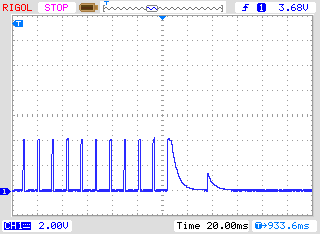
\includegraphics[]{../PNG/IRFU120gate.png}
\caption{measuring of threshold voltage of N-Channel-MOSFET}
\label{fig:eleven}
\end{figure}

\subsection{Measurement of Diodes}
\label{sec:diode}
If current is detected with the pre-tests, the behavior of the part will be checked to
be a diode. The flow voltage with the \(680\Omega\) resistor must be between 0.15V and 4.64V.
The flux voltage with the \(680\Omega\) must be greater than 1.125 times the flux voltage with
the \(470k\Omega\) resistor and eight times the flux voltage with the \(470k\Omega\) must be
greater than the flux voltage with the \(680\Omega\) resistor.
I hope, that this behavior is always a diode.

\subsection{Results of different measurements}
The following three tables shows results of different test probes with different
software configurations with the ATmega8 and ATmega168 processors.

\begin{table}[H]
  \begin{center}
    \begin{tabular}{| l | c | c | c |}
    \hline
     Diode & Mega8@8MHz & Mega168 @8MHz & Mega168 @8MHz \\
     Type  & signature 1E9307 & signature 1E9406 & signature 1E9406 \\
           & WITH\_AUTO\_REF &  & WITH\_AUTO\_REF \\
           &                 &  & AUTOSCALE\_ADC \\
    \hline
    \hline
1N4148 & Diode, 721mV, 0pF & Diode, 729mV, 0pF & Diode, 725mV, 0pF\\
    \hline
1N4150 & Diode, 678mV, 0pF & Diode, 681mV, 0pF & Diode, 682mV, 0pF\\
    \hline
BA157 & Diode,623mV, 17pF & Diode, 631mV, 16pF & Diode, 620mV, 15pF\\
    \hline
BY398 & Diode, 541mV, 0pF & Diode, 553mV, 0pF & Diode, 542mV, 0pF\\
    \hline
1N4007 & Diode, 654mV, 13pF & Diode, 665mV, 9pF & Diode, 658mV, 11pF\\
    \hline
LED green & Diode, 1954mV, 6pF & Diode, 1970mV, 6pF & Diode, 1951mV, 4pF\\
    \hline
ZPD2,7 & 2xDi, 729mV, 2659mV & 2xDi, 738mV, 2674mV & 2xDi, 730mV, 2656mV \\
    \hline
BU508A B+E & Diode, 613mV, 5201pF & Diode, 621mV, 5285pF & Diode, 611mV, 5344pF\\
    \hline
BU508A B+C & Diode, 595mV, 261pF & Diode, 597mV, 267pF & Diode, 591mV, 272pF\\
    \hline
    \end{tabular}
  \end{center}
  \caption{measurement results of diode testing}
  \label{tab:diodes} 
\end{table}

\begin{table}[H]
  \begin{center}
    \begin{tabular}{| l | c | c | c |}
    \hline
     Transistor & Mega8@8MHz & Mega168 @8MHz & Mega168 @8MHz \\
     Type   & signature 1E9307 & signature 1E9406 & signature 1E9406 \\
           & WITH\_AUTO\_REF &  & WITH\_AUTO\_REF \\
           &                 &  & AUTOSCALE\_ADC \\
    \hline
    \hline
BU508A & NPN, B=9, 613mV & NPN, B=9, 621mV & NPN, B=9, 615mV\\
    \hline
2N3055 & NPN, B=21, 617mV & NPN, B=21, 626mV & NPN, B=21, 625mV\\
    \hline
BC546B & NPN, B=381, 780mV & NPN, B=376, 777mV & NPN, B=387, 771mV\\
    \hline
BC556B & PNP, B=266, 790mV & PNP, B=429, 787mV & PNP, B=266, 790mV\\
    \hline
BC639 & NPN, B=180, 722mV & NPN, B=180, 733mV & NPN, B=188, 724mV\\

    \hline
BC640 & PNP, B=185, 716mV & PNP, B=227, 725mV & PNP, B=187, 719mV\\
    \hline
AC128 (Ge.) & PNP, B=68, 270mV & PNP, B=64, 269mV & PNP, B=66, 271mV\\
    \hline
BC517 & NPN, B=26996, 1419mV & NPN, B=28220, 1413mV & NPN, B=28250, 1404mV\\
    \hline
BC516 & PNP, B=65535, 1430mV & PNP, B=65535, 1420mV & PNP, B=65535, 1417mV\\
    \hline
BRY55/200 & Thyristor & Thyristor & Thyristor\\
    \hline
    \end{tabular}
  \end{center}
  \caption{measurement results of bipolar transistor testing}
  \label{tab:bipolar} 
\end{table}

\begin{table}[H]
  \begin{center}
    \begin{tabular}{| l | c | c | c |}
    \hline
     FET & Mega8@8MHz & Mega168 @8MHz & Mega168 @8MHz \\
    Type    & signature 1E9307 & signature 1E9406 & signature 1E9406 \\
           & WITH\_AUTO\_REF &  & WITH\_AUTO\_REF \\
           &                 &  & AUTOSCALE\_ADC \\
    \hline
    \hline
BS170 & N-E-MOS,D, 2616mV & N-E-MOS,D, 2562mV & N-E-MOS,D, 2564mV \\
      &  66pF             &  67pF  &  68pF \\
    \hline
J310 & N-JFET & N-JFET & N-JFET\\
    \hline
IRFU120N & N-E-MOS,D, 4151mV & N-E-MOS,D, 4156mV & N-E-MOS,D, 4153mV\\
     & 922pF  & 894pF  & 933pF \\
    \hline
IRFU9024 & P-E-MOS,D, 3525mV & P-E-MOS,D, 3525mV & P-E-MOS,D, 3534mV\\
     & 960pF & 926pF & 965pF \\
    \hline
ZVP2106A & P-E-MOS,D, 3217mV & P-E-MOS,D, 3220mV & P-E-MOS,D, 3217mV\\
  & 115pF & 114pF & 113pF \\
    \hline
ZVNL120A & N-E-MOS,D, 1560mV & N-E-MOS,D, 1535mV & N-E-MOS,D, 1535mV \\
  & 140pF & 138pF  & 138pF \\
    \hline
    \end{tabular}
  \end{center}
  \caption{measurement results of MOS transistor testing}
  \label{tab:mos} 
\end{table}
